\chapter{System Design and Architechure}
System design is the process of designing the elements of a system such as the architecture, modules and components, the different interfaces of those components and the data that goes through that system.

\section{Use Cases}
\begin{figure}[H]
    \centering
    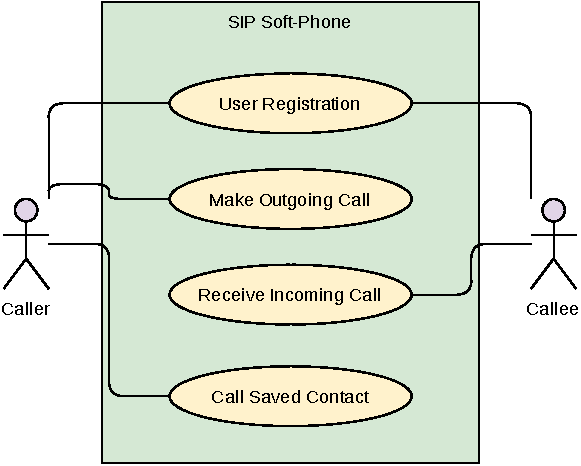
\includegraphics{UseCase}
    \caption{Use Case Diagram}
    \label{fig:use_case}
\end{figure}

\section{Activity Diagrams}
An activity diagram is a behavioral diagram i.e. it depicts the behavior of a system. An activity diagram portrays the control flow from a start point to a finish point showing the various decision paths that exist while the activity is being executed.

\subsection{User Registration}
\begin{figure}[H]
    \centering
    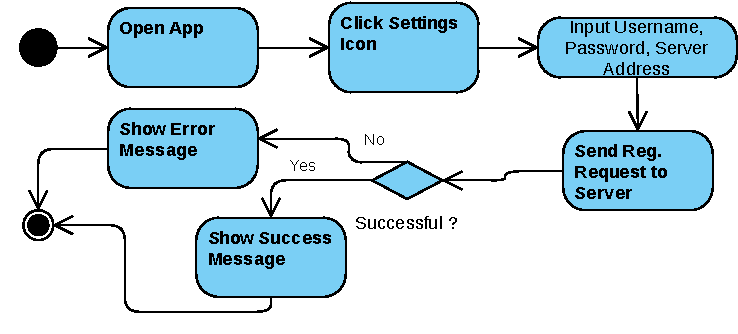
\includegraphics{RegActivity}
    \caption{Activity Diagram for SIP User Registration}
    \label{fig:reg_activity}
\end{figure}

\subsection{Make Outgoing Call}
\begin{figure}[H]
    \centering
    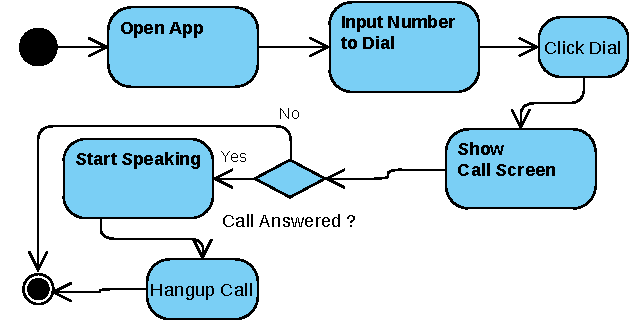
\includegraphics{OutgoingActivity}
    \caption{Activity Diagram for Outgoing Calls}
    \label{fig:out_activity}
\end{figure}

\subsection{Receive Incoming Call}
\begin{figure}[H]
    \centering
    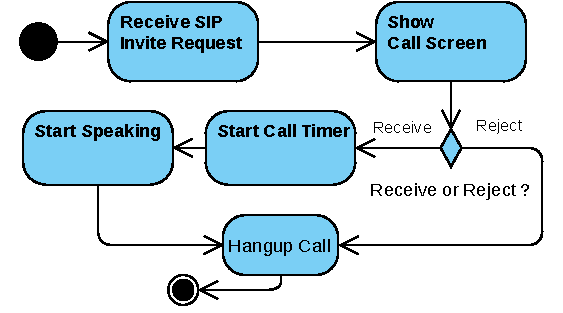
\includegraphics{ReceiveActivity}
    \caption{Activity Diagram for Incoming Calls}
    \label{fig:recv_activity}
\end{figure}

\subsection{Call a Saved Contact}
\begin{figure}[H]
    \centering
    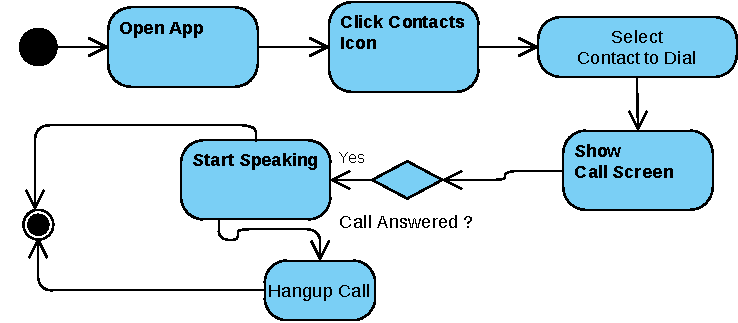
\includegraphics{SavedActivity}
    \caption{Activity Diagram for Calling a Saved Contact}
    \label{fig:saved_activity}
\end{figure}
\clearpage

\section{Class Diagrams}
A class diagram is a diagram used in designing and modeling software to describe classes and their relationships.

\subsection{Classes and Their Properties}
\begin{figure}[H]
    \centering
    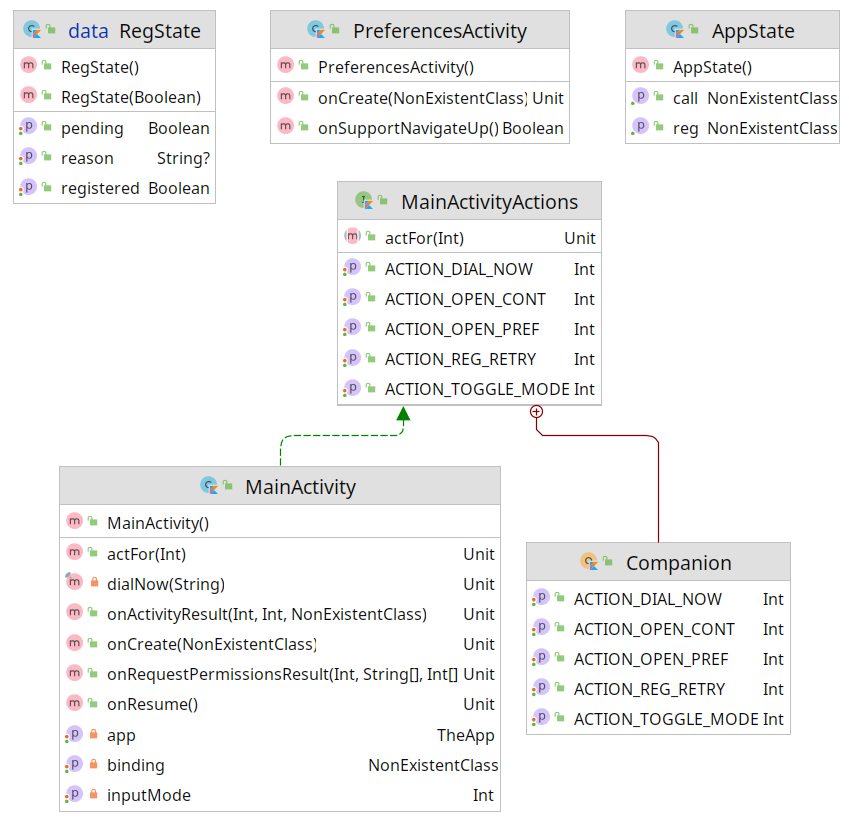
\includegraphics[width=\textwidth]{cd-1}
\end{figure}
\clearpage
\begin{figure}[H]
    \centering
    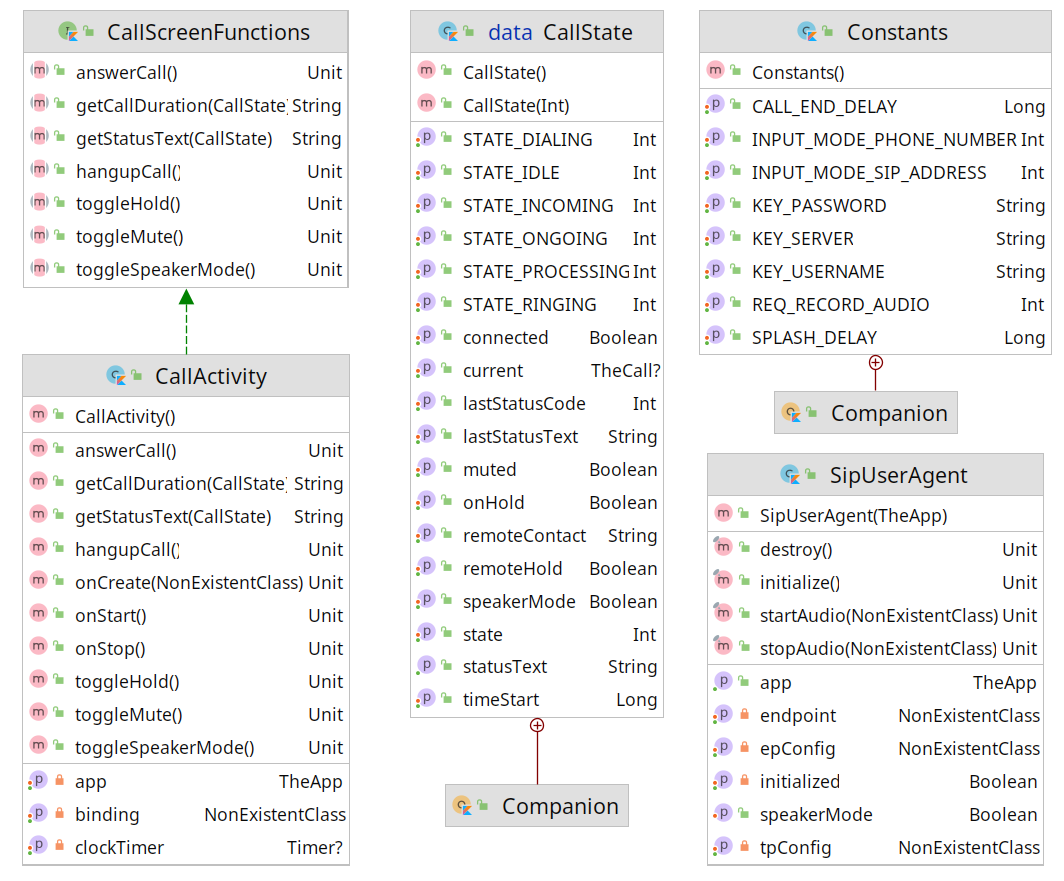
\includegraphics[width=\textwidth]{cd-2}
\end{figure}
\clearpage
\begin{figure}[H]
    \centering
    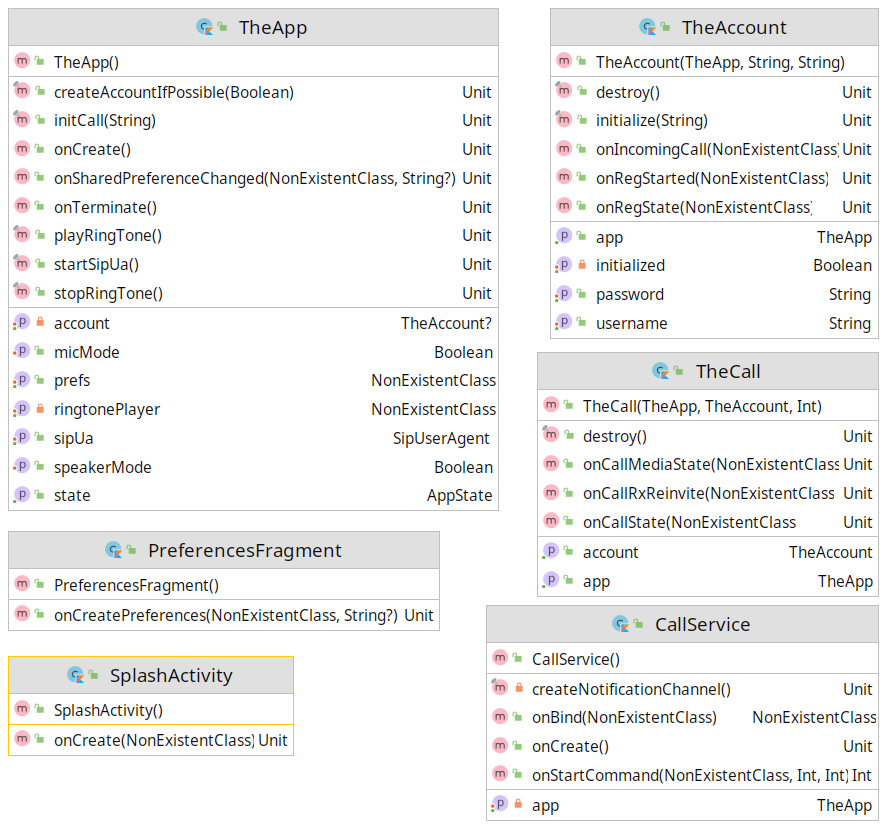
\includegraphics[width=\textwidth]{cd-3}
    \caption{Classes and Their Properties}
    \label{fig:class-props}
\end{figure}
\clearpage
\subsection{Class Dependencies}
\begin{figure}[H]
    \centering
    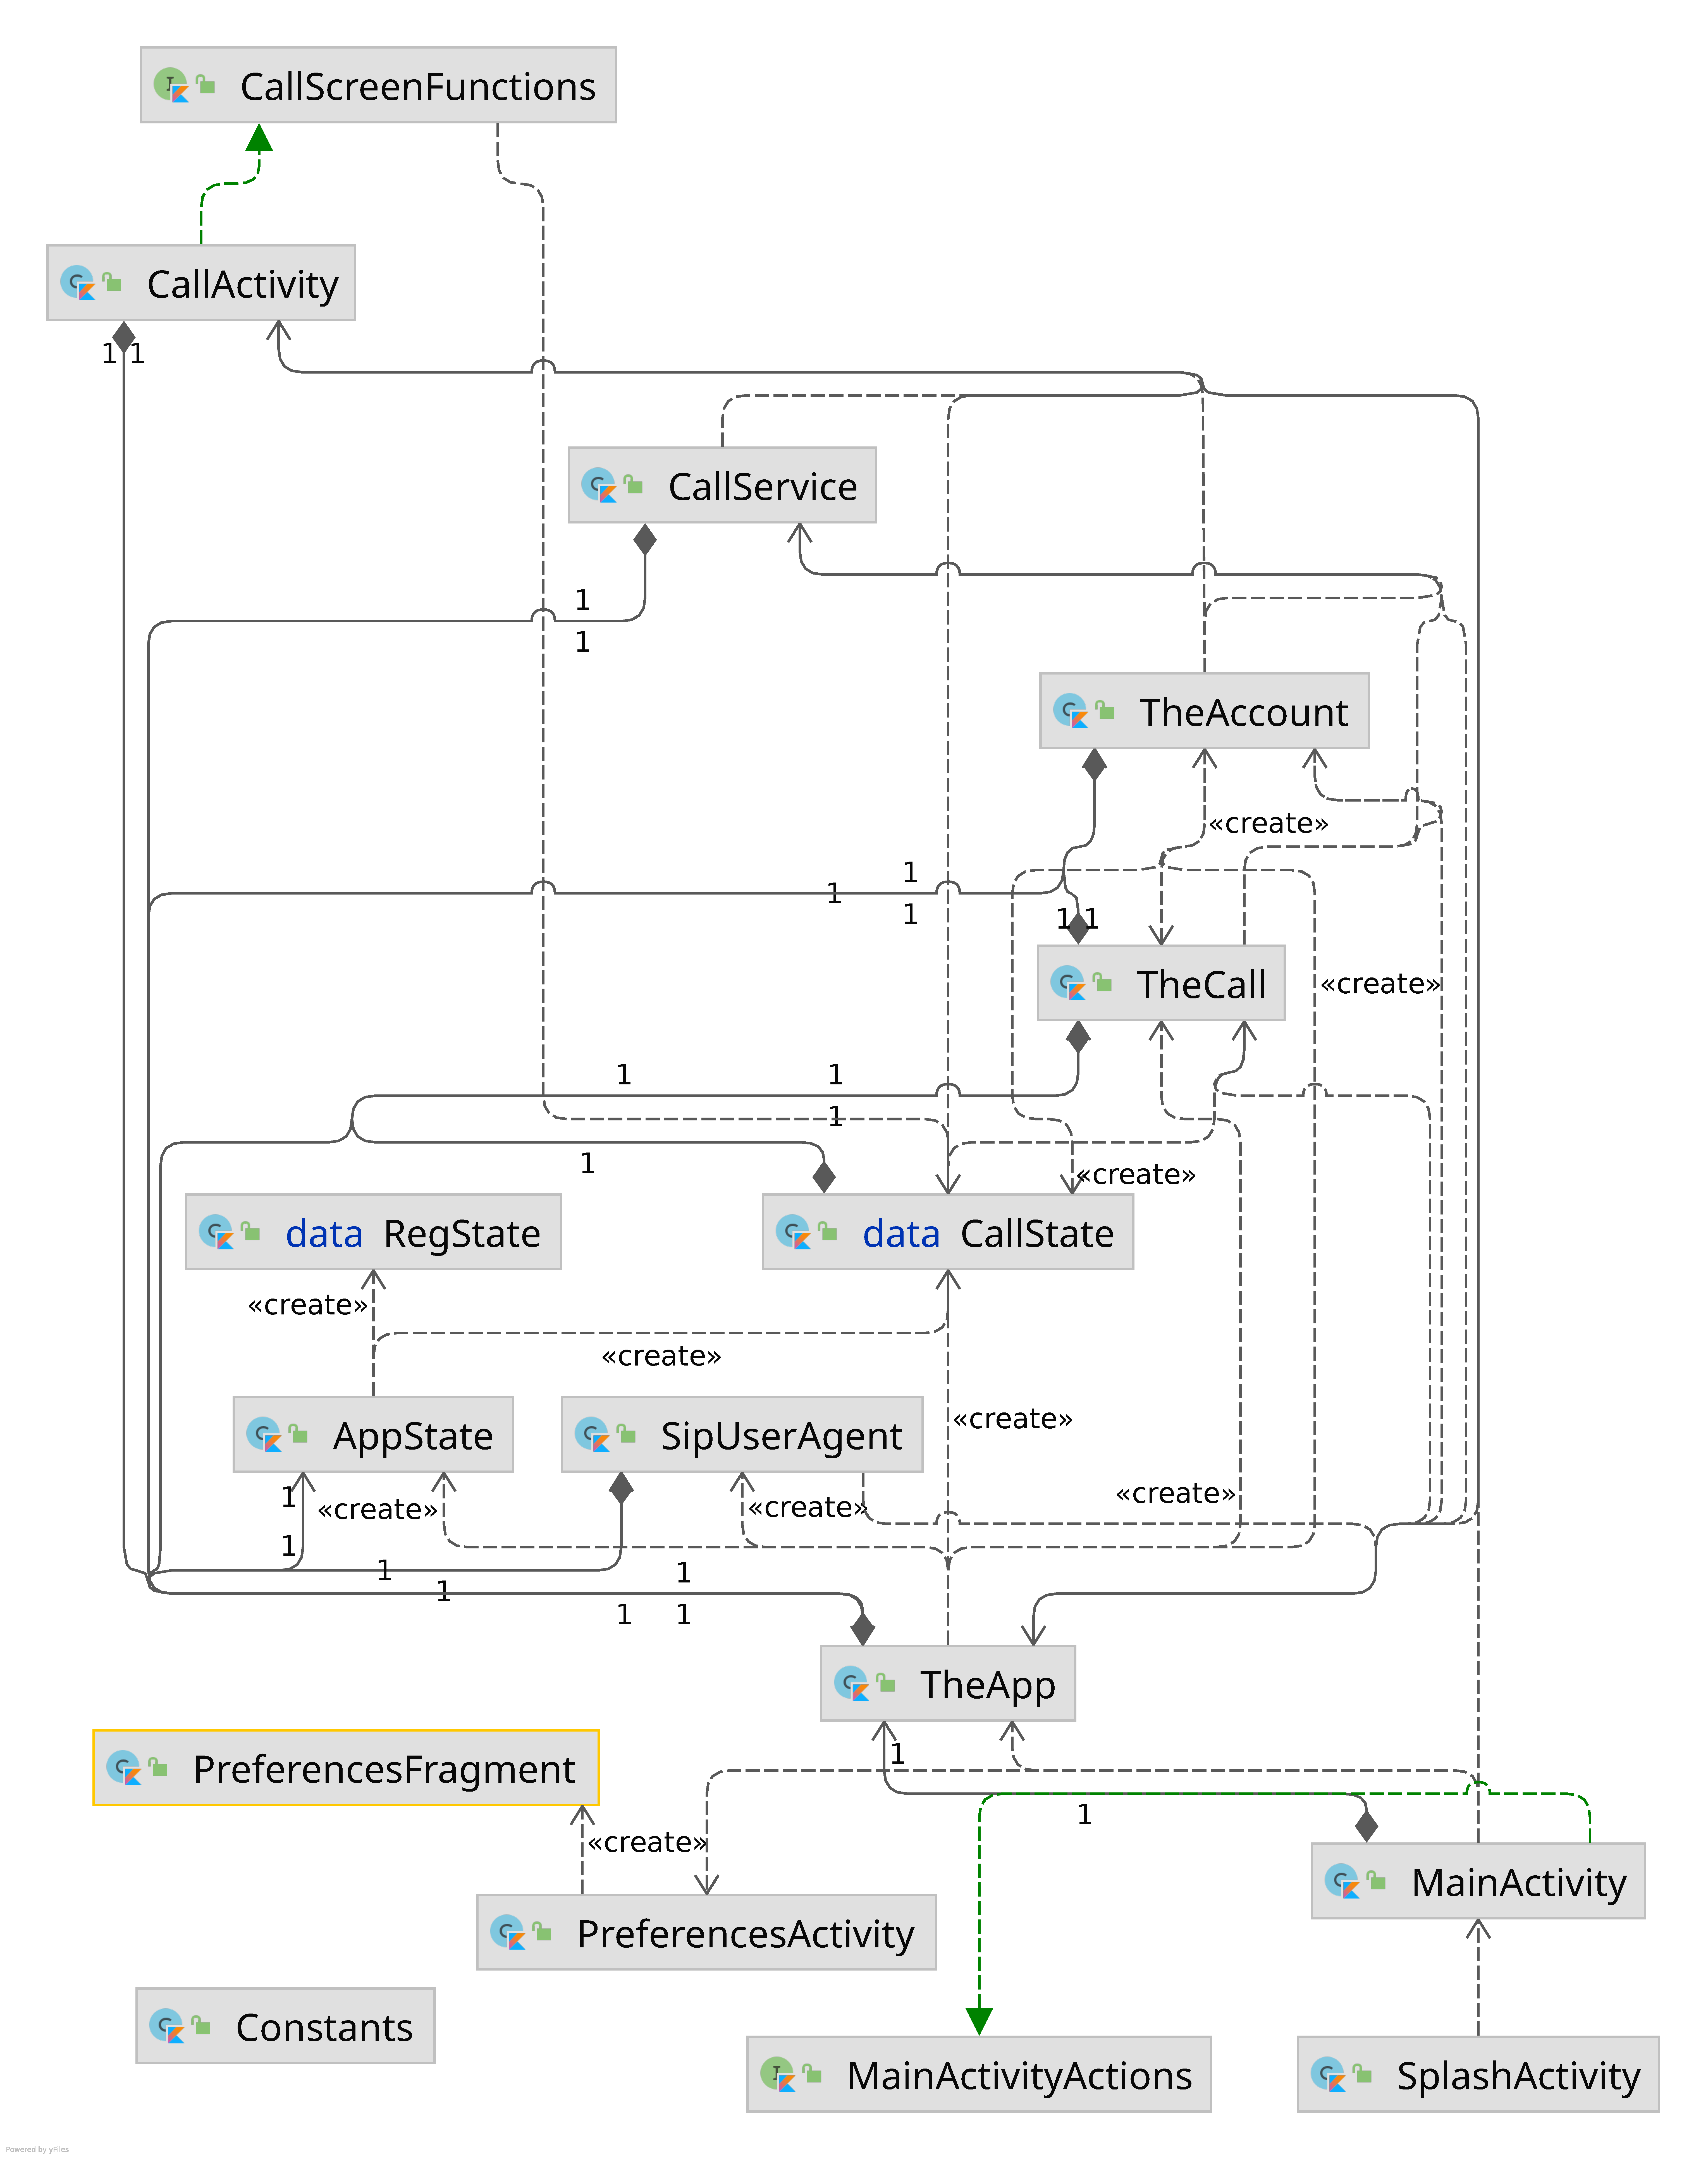
\includegraphics[height=.85\textheight]{class-deps}
    \caption{Class Dependencies and Relationships}
    \label{fig:class-dep}
\end{figure}
\clearpage

\section{User Interface Prototypes}
Prototypes are a close replica of what the end result of a product will look like, usually without code. They incorporate most of the final UI design and interaction that the finished product will have. Prototyping is one of the most powerful tools in a UX designer's inventory.
\\ \\
We have designed following UI prototypes:
\begin{enumerate}
 \item Application's Home Screen
 \item App Settings Screen
 \item Incoming Call Screen
 \item Active In-Call Screen
\end{enumerate}

\subsection{App Home Screen}
\begin{figure}[H]
    \centering
    \frame{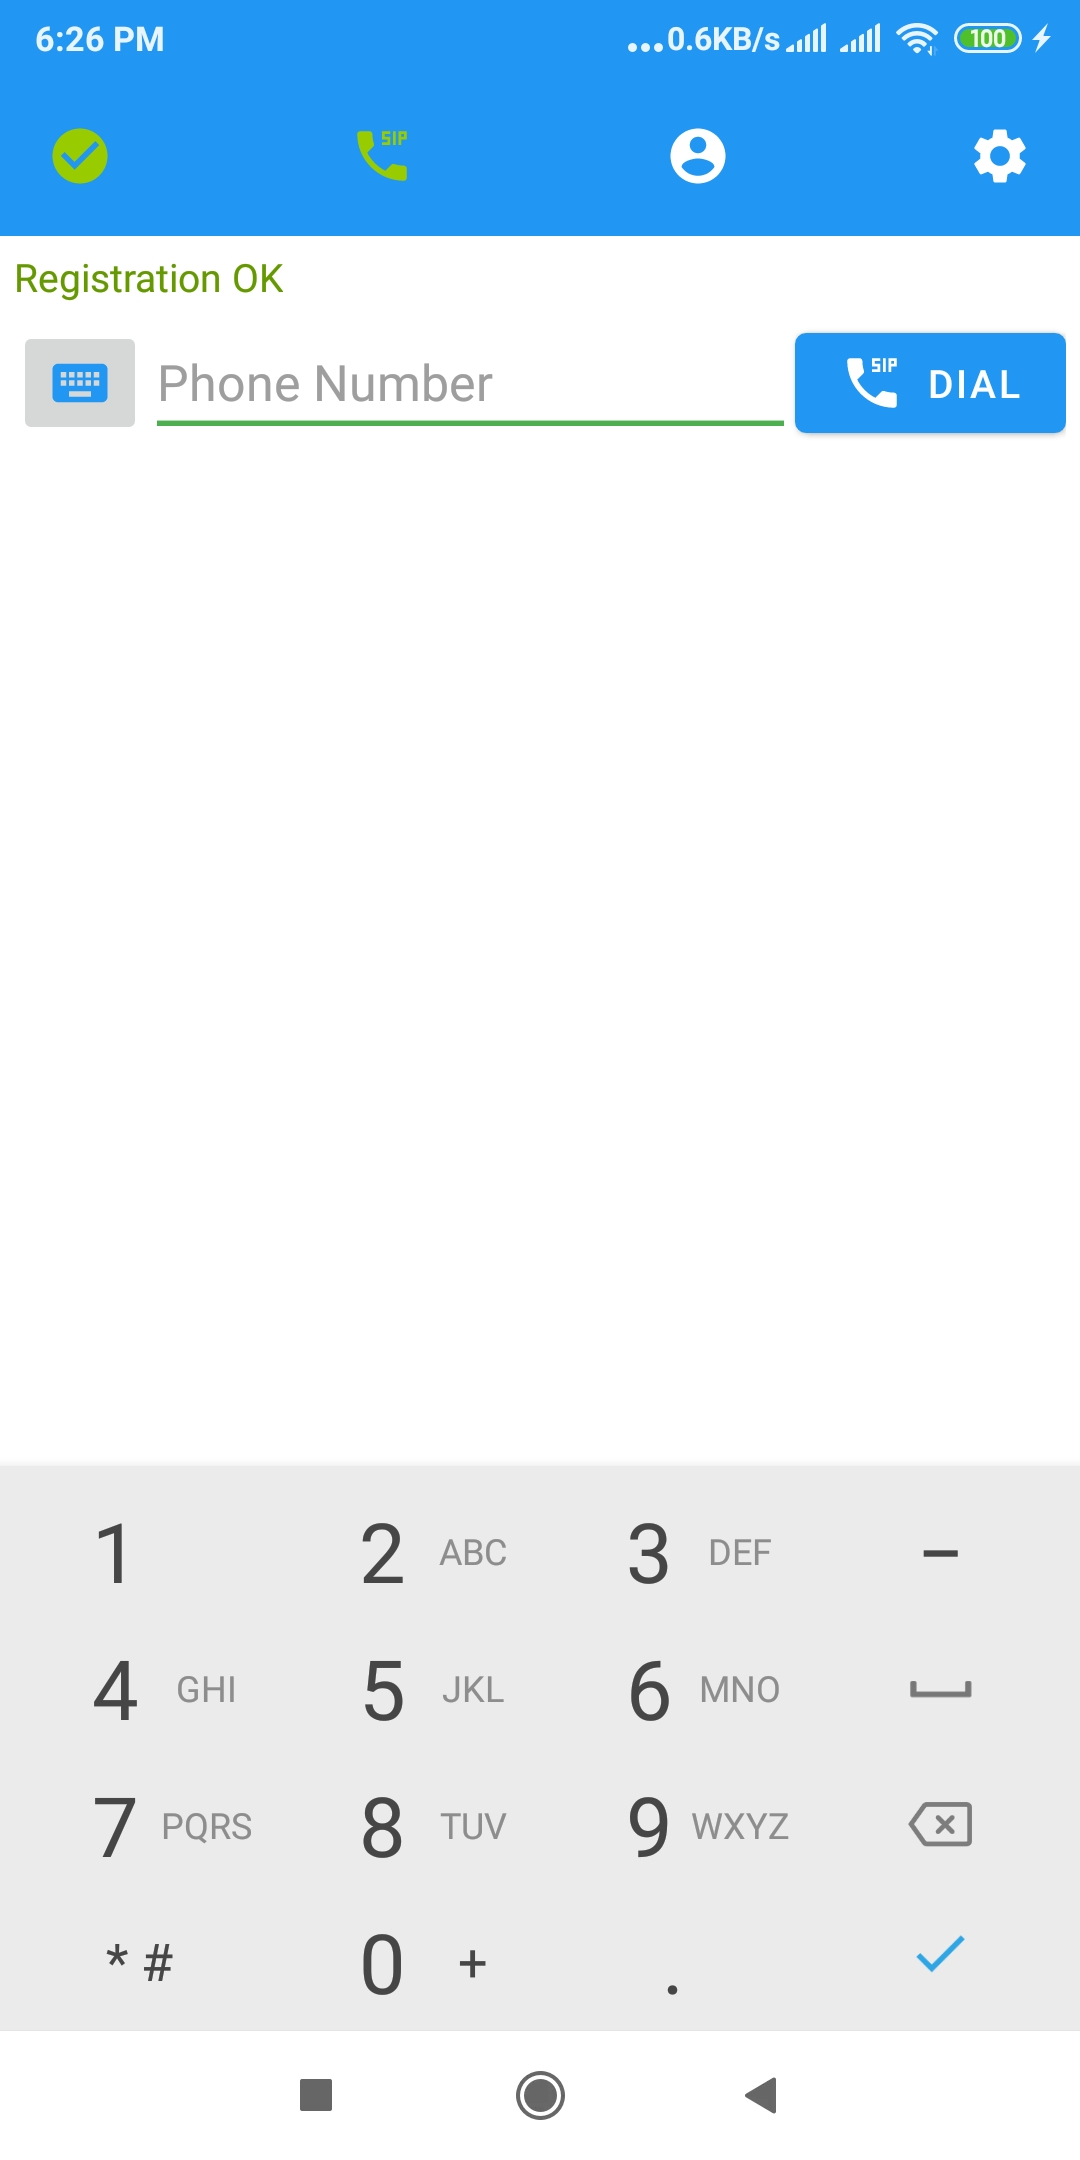
\includegraphics[width=.65\textwidth]{home}}
    \caption{UI Prototype of App Home Screen}
    \label{fig:app_home}
\end{figure}

\subsection{Settings Screen}
\begin{figure}[H]
    \centering
    \frame{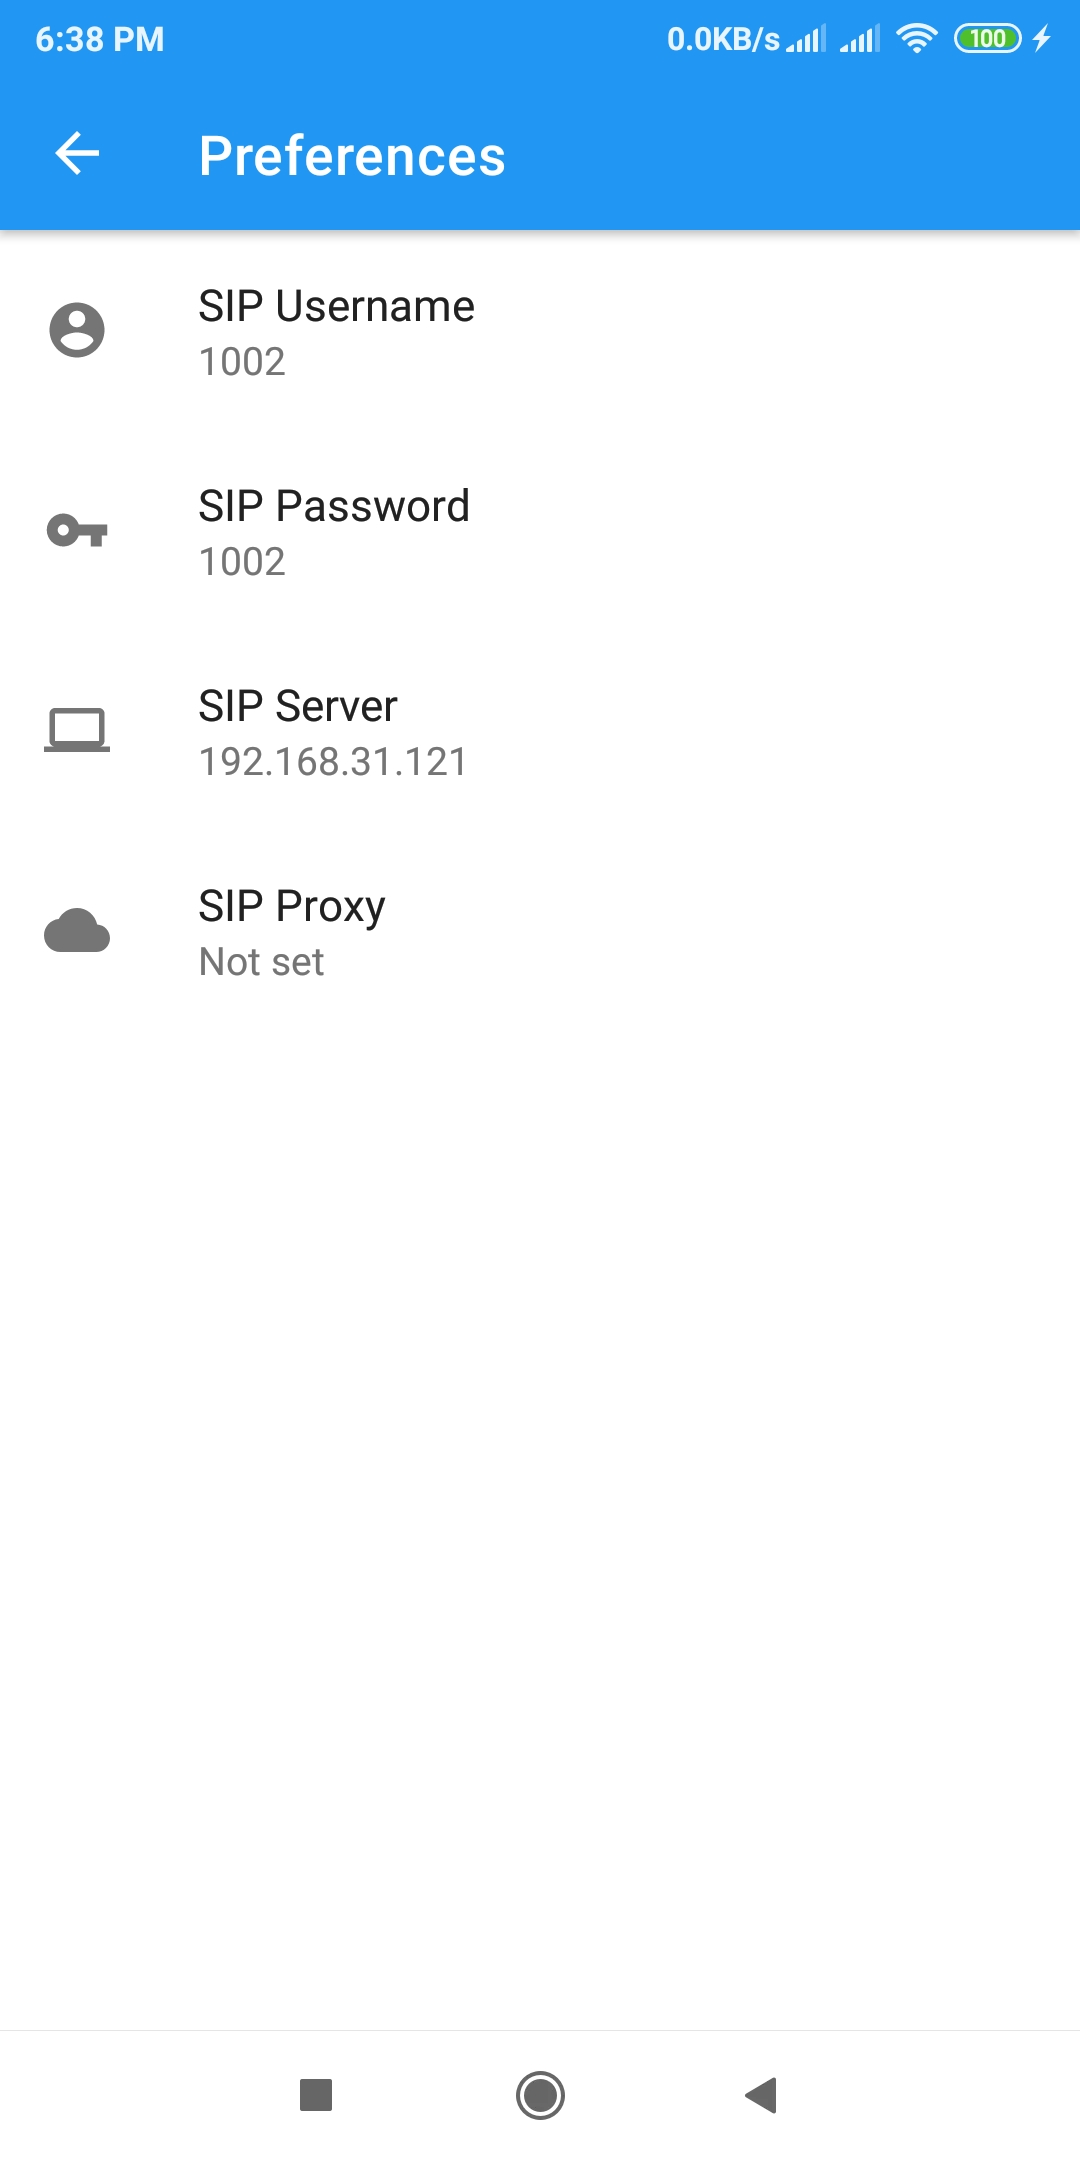
\includegraphics[width=.65\textwidth]{settings}}
    \caption{UI Prototype of Settings Screen}
    \label{fig:app_set}
\end{figure}

\subsection{Incoming Call Screen}
\begin{figure}[H]
    \centering
    \frame{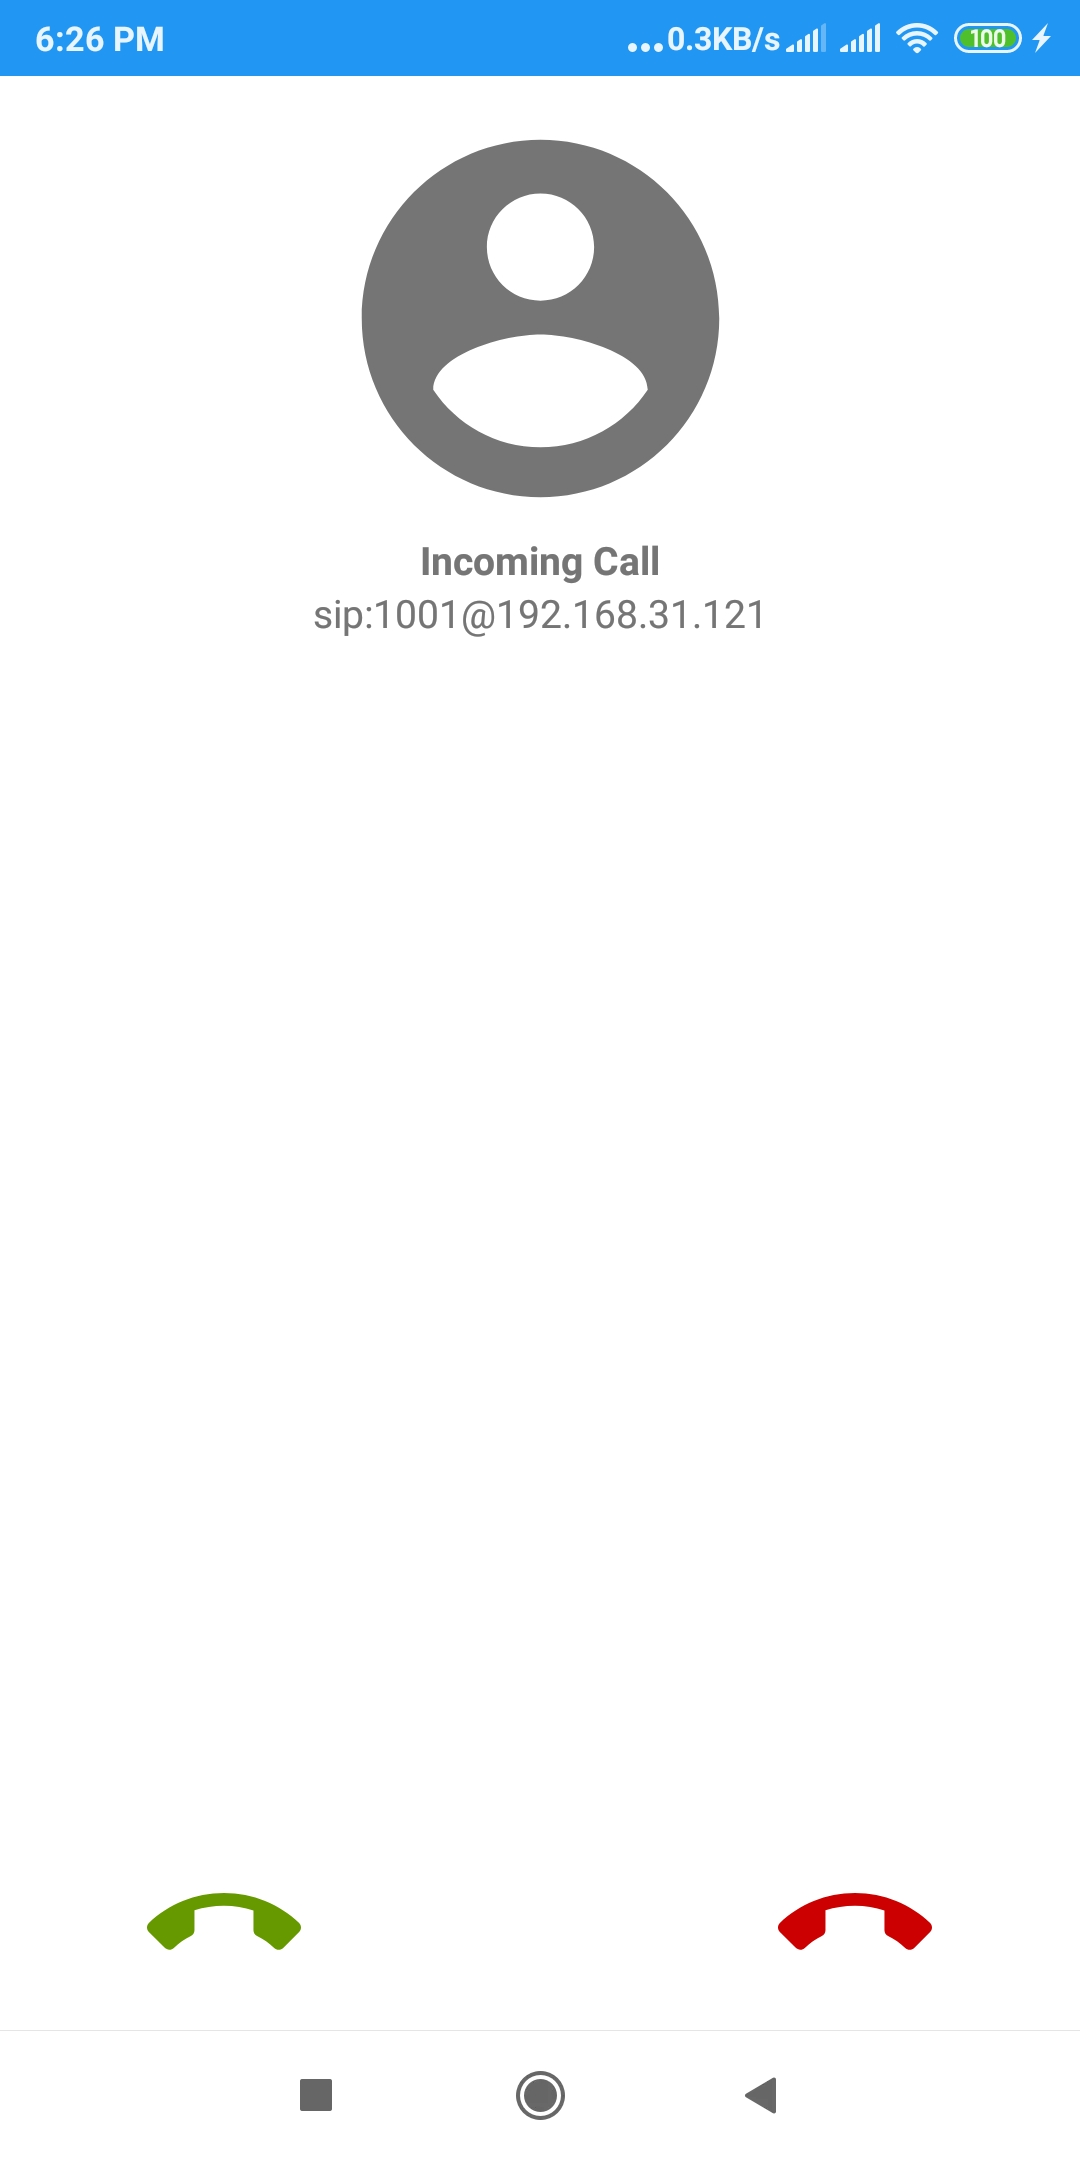
\includegraphics[width=.65\textwidth]{incoming}}
    \caption{UI Prototype of Incoming Call Screen}
    \label{fig:app_incoming}
\end{figure}

\subsection{Active Call Screen}
\begin{figure}[H]
    \centering
    \frame{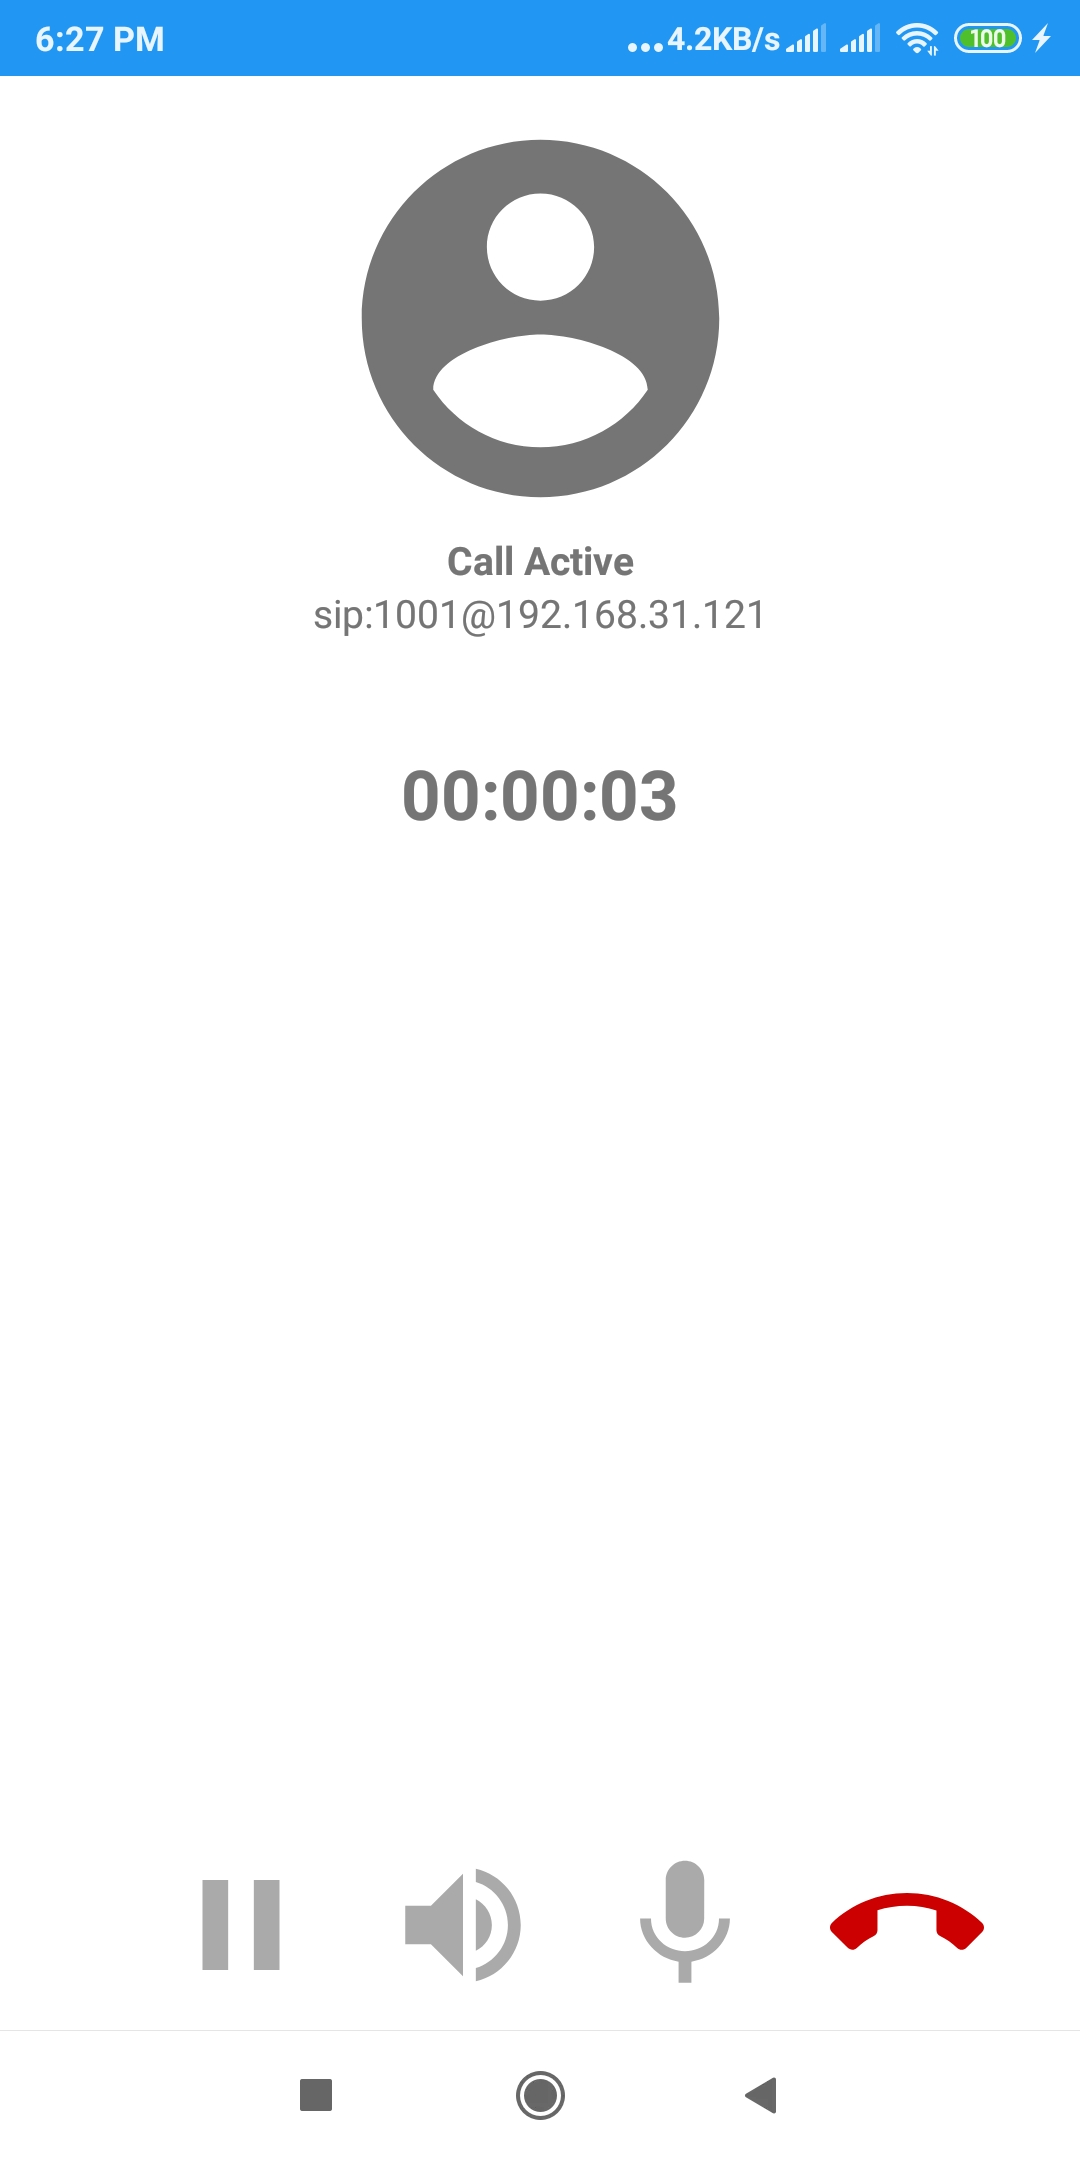
\includegraphics[width=.65\textwidth]{in-call}}
    \caption{UI Prototype of Active Call Screen}
    \label{fig:app_in_call}
\end{figure}
